\documentclass{book}
\usepackage[a4paper,top=2.5cm,bottom=2.5cm,left=2.5cm,right=2.5cm]{geometry}
\usepackage{makeidx}
\usepackage{natbib}
\usepackage{graphicx}
\usepackage{multicol}
\usepackage{float}
\usepackage{listings}
\usepackage{color}
\usepackage{ifthen}
\usepackage[table]{xcolor}
\usepackage{textcomp}
\usepackage{alltt}
\usepackage{ifpdf}
\ifpdf
\usepackage[pdftex,
            pagebackref=true,
            colorlinks=true,
            linkcolor=blue,
            unicode
           ]{hyperref}
\else
\usepackage[ps2pdf,
            pagebackref=true,
            colorlinks=true,
            linkcolor=blue,
            unicode
           ]{hyperref}
\usepackage{pspicture}
\fi
\usepackage[utf8]{inputenc}
\usepackage{mathptmx}
\usepackage[scaled=.90]{helvet}
\usepackage{courier}
\usepackage{sectsty}
\usepackage{amssymb}
\usepackage[titles]{tocloft}
\usepackage{doxygen}
\lstset{language=C++,inputencoding=utf8,basicstyle=\footnotesize,breaklines=true,breakatwhitespace=true,tabsize=4,numbers=left }
\makeindex
\setcounter{tocdepth}{3}
\renewcommand{\footrulewidth}{0.4pt}
\renewcommand{\familydefault}{\sfdefault}
\hfuzz=15pt
\setlength{\emergencystretch}{15pt}
\hbadness=750
\tolerance=750
\begin{document}
\hypersetup{pageanchor=false,citecolor=blue}
\begin{titlepage}
\vspace*{7cm}
\begin{center}
{\Large My Project }\\
\vspace*{1cm}
{\large Generated by Doxygen 1.8.2}\\
\vspace*{0.5cm}
{\small Mon Mar 4 2013 10:35:26}\\
\end{center}
\end{titlepage}
\clearemptydoublepage
\pagenumbering{roman}
\tableofcontents
\clearemptydoublepage
\pagenumbering{arabic}
\hypersetup{pageanchor=true,citecolor=blue}
\chapter{Hierarchical Index}
\section{Class Hierarchy}
This inheritance list is sorted roughly, but not completely, alphabetically\-:\begin{DoxyCompactList}
\item Coment\-Protocol\begin{DoxyCompactList}
\item \contentsline{section}{L\-N\-Coment}{\pageref{class_l_n_coment}}{}
\end{DoxyCompactList}
\item \contentsline{section}{Initial\-I\-U\-Controler}{\pageref{class_initial_i_u_controler}}{}
\item \contentsline{section}{I\-U\-Coment\-Protocol}{\pageref{class_i_u_coment_protocol}}{}
\begin{DoxyCompactList}
\item \contentsline{section}{Coment\-Controler}{\pageref{class_coment_controler}}{}
\end{DoxyCompactList}
\item \contentsline{section}{I\-U\-Post\-Protocol}{\pageref{class_i_u_post_protocol}}{}
\begin{DoxyCompactList}
\item \contentsline{section}{Post\-Controler}{\pageref{class_post_controler}}{}
\end{DoxyCompactList}
\item \contentsline{section}{I\-U\-User\-Protocol}{\pageref{class_i_u_user_protocol}}{}
\begin{DoxyCompactList}
\item \contentsline{section}{User\-Controler}{\pageref{class_user_controler}}{}
\end{DoxyCompactList}
\item Post\-Protocol\begin{DoxyCompactList}
\item \contentsline{section}{L\-N\-Post}{\pageref{class_l_n_post}}{}
\end{DoxyCompactList}
\item User\-Protocol\begin{DoxyCompactList}
\item \contentsline{section}{L\-N\-User}{\pageref{class_l_n_user}}{}
\end{DoxyCompactList}
\end{DoxyCompactList}

\chapter{Class Index}
\section{Class List}
Here are the classes, structs, unions and interfaces with brief descriptions\-:\begin{DoxyCompactList}
\item\contentsline{section}{\hyperlink{class_coment_controler}{Coment\-Controler} \\*Essa é a classe que cria a interface de comandos de comentário }{\pageref{class_coment_controler}}{}
\item\contentsline{section}{\hyperlink{class_initial_i_u_controler}{Initial\-I\-U\-Controler} \\*Essa é a classe que cria a primeira interface que conecta as intefarces para comando de usuário, post e comentário }{\pageref{class_initial_i_u_controler}}{}
\item\contentsline{section}{\hyperlink{class_i_u_coment_protocol}{I\-U\-Coment\-Protocol} \\*Essa é a classe abstrata que gera os métodos que serão usados pelos protocolos de interface }{\pageref{class_i_u_coment_protocol}}{}
\item\contentsline{section}{\hyperlink{class_i_u_post_protocol}{I\-U\-Post\-Protocol} \\*Essa é a classe abstrata que gera os métodos que serão usados pelos protocolos de interface }{\pageref{class_i_u_post_protocol}}{}
\item\contentsline{section}{\hyperlink{class_i_u_user_protocol}{I\-U\-User\-Protocol} \\*Essa é a classe abstrata que gera os métodos que serão usados pelos protocolos de interface }{\pageref{class_i_u_user_protocol}}{}
\item\contentsline{section}{\hyperlink{class_l_n_coment}{L\-N\-Coment} }{\pageref{class_l_n_coment}}{}
\item\contentsline{section}{\hyperlink{class_l_n_post}{L\-N\-Post} }{\pageref{class_l_n_post}}{}
\item\contentsline{section}{\hyperlink{class_l_n_user}{L\-N\-User} \\*Essa � a classe respons�vel pela l�gica de neg�cios para uma postagems }{\pageref{class_l_n_user}}{}
\item\contentsline{section}{\hyperlink{class_post_controler}{Post\-Controler} \\*Essa é a classe que cria a interface de comandos de post }{\pageref{class_post_controler}}{}
\item\contentsline{section}{\hyperlink{class_user_controler}{User\-Controler} \\*Essa é a classe que cria a interface de comandos de usuário }{\pageref{class_user_controler}}{}
\end{DoxyCompactList}

\chapter{File Index}
\section{File List}
Here is a list of all documented files with brief descriptions\-:\begin{DoxyCompactList}
\item\contentsline{section}{{\bfseries Inter\-Usu.\-h} }{\pageref{_inter_usu_8h}}{}
\item\contentsline{section}{\hyperlink{_i_u_protocols_8h}{I\-U\-Protocols.\-h} \\*Este e o cabecalho do modulo das classes entidades que definem as \par
 entidades do sistema neste caso estes sao\-:\par
 }{\pageref{_i_u_protocols_8h}}{}
\end{DoxyCompactList}

\chapter{Class Documentation}
\hypertarget{class_coment_protocol}{\section{Coment\-Protocol Class Reference}
\label{class_coment_protocol}\index{Coment\-Protocol@{Coment\-Protocol}}
}


Inheritance diagram for Coment\-Protocol\-:\nopagebreak
\begin{figure}[H]
\begin{center}
\leavevmode
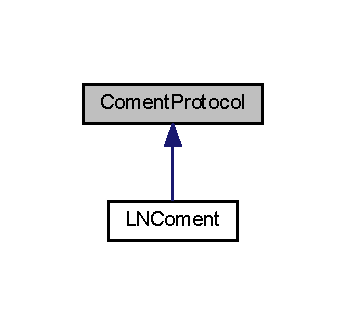
\includegraphics[width=166pt]{class_coment_protocol__inherit__graph}
\end{center}
\end{figure}
\subsection*{Public Member Functions}
\begin{DoxyCompactItemize}
\item 
\hypertarget{class_coment_protocol_a96c2e0cb9eb4fdbf5a7eae853b6546df}{virtual void {\bfseries novo} (\hyperlink{class_coment}{Coment})=0}\label{class_coment_protocol_a96c2e0cb9eb4fdbf5a7eae853b6546df}

\item 
\hypertarget{class_coment_protocol_a5a1cc6af2c1a52b489e6897070e4183a}{virtual void {\bfseries update} (\hyperlink{class_coment}{Coment})=0}\label{class_coment_protocol_a5a1cc6af2c1a52b489e6897070e4183a}

\item 
\hypertarget{class_coment_protocol_a466292c4e836394ce7a46a9b86412cae}{virtual void {\bfseries deleta} (\hyperlink{class_coment}{Coment})=0}\label{class_coment_protocol_a466292c4e836394ce7a46a9b86412cae}

\item 
\hypertarget{class_coment_protocol_a3a1f008a4638d4d1505b416d7e866158}{virtual \hyperlink{class_coment}{Coment} {\bfseries pegar} (\hyperlink{class_coment}{Coment})=0}\label{class_coment_protocol_a3a1f008a4638d4d1505b416d7e866158}

\item 
\hypertarget{class_coment_protocol_af626d6d87a2586d33d8fdfbab674ea1a}{virtual list$<$ \hyperlink{class_coment}{Coment} $>$ {\bfseries listar} (\hyperlink{class_coment}{Coment})=0}\label{class_coment_protocol_af626d6d87a2586d33d8fdfbab674ea1a}

\item 
\hypertarget{class_coment_protocol_a282b789ce1d561b29a3eb68af1de7296}{virtual void {\bfseries set\-Percistence} (\hyperlink{class_percistence_protocol}{Percistence\-Protocol} $\ast$)=0}\label{class_coment_protocol_a282b789ce1d561b29a3eb68af1de7296}

\end{DoxyCompactItemize}


The documentation for this class was generated from the following file\-:\begin{DoxyCompactItemize}
\item 
C\-:/\-Users/\-Vitor/\-Desktop/\-Work\-Space/\-P\-R\-O\-J\-E\-T\-O\-\_\-\-F\-I\-N\-A\-L\-\_\-\-P\-O\-O/\-P\-R\-O\-J\-E\-T\-O\-\_\-\-D\-E\-V/\-P\-R\-O\-J\-E\-T\-O/\-Projeto\-\_\-codeblocks/\hyperlink{_protocolo_l_n_8h}{Protocolo\-L\-N.\-h}\end{DoxyCompactItemize}

\hypertarget{class_l_n_coment}{\section{L\-N\-Coment Class Reference}
\label{class_l_n_coment}\index{L\-N\-Coment@{L\-N\-Coment}}
}


Inheritance diagram for L\-N\-Coment\-:
\nopagebreak
\begin{figure}[H]
\begin{center}
\leavevmode
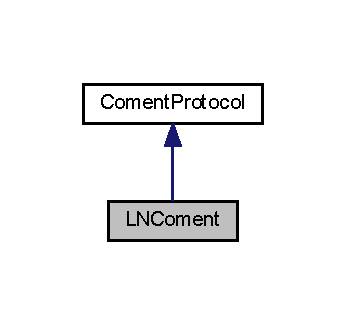
\includegraphics[width=166pt]{class_l_n_coment__inherit__graph}
\end{center}
\end{figure}


Collaboration diagram for L\-N\-Coment\-:
\nopagebreak
\begin{figure}[H]
\begin{center}
\leavevmode
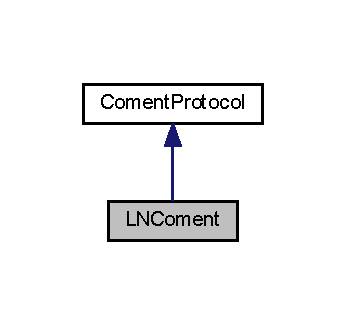
\includegraphics[width=166pt]{class_l_n_coment__coll__graph}
\end{center}
\end{figure}
\subsection*{Public Member Functions}
\begin{DoxyCompactItemize}
\item 
void \hyperlink{class_l_n_coment_a0c4839930f9a6d65f6200845fdab9750}{novo} (Coment)
\begin{DoxyCompactList}\small\item\em M�todo respons�vel por criar uma coment�rio. \end{DoxyCompactList}\item 
void \hyperlink{class_l_n_coment_acefe80ac606f9258093f22eca0759cb0}{update} (Coment)
\begin{DoxyCompactList}\small\item\em M�todo respons�vel por atualizar um coment�rio. \end{DoxyCompactList}\item 
void \hyperlink{class_l_n_coment_abf2ff1565521a03e001ff907eeec7fe9}{deleta} (Coment)
\begin{DoxyCompactList}\small\item\em M�todo respons�vel por deletar uma coment�rio. \end{DoxyCompactList}\item 
Coment \hyperlink{class_l_n_coment_a321fb89a92d2af289267c0ccac1c090f}{pegar} (Coment)
\begin{DoxyCompactList}\small\item\em M�todo respons�vel por pegar uma coment�rio. \end{DoxyCompactList}\item 
list$<$ Coment $>$ \hyperlink{class_l_n_coment_aebcc6610b6b288196ce101440a817c3d}{listar} ()
\begin{DoxyCompactList}\small\item\em M�todo respons�vel por listar todos os coment�rios de um post. \end{DoxyCompactList}\item 
virtual void \hyperlink{class_l_n_coment_abdf75faf2dc51482a09958f78095b008}{set\-Percistence} (Percistence\-Protocol $\ast$)
\begin{DoxyCompactList}\small\item\em M�todo respons�vel por ativar um protocolo de persit�ncia. \end{DoxyCompactList}\end{DoxyCompactItemize}


\subsection{Member Function Documentation}
\hypertarget{class_l_n_coment_abf2ff1565521a03e001ff907eeec7fe9}{\index{L\-N\-Coment@{L\-N\-Coment}!deleta@{deleta}}
\index{deleta@{deleta}!LNComent@{L\-N\-Coment}}
\subsubsection[{deleta}]{\setlength{\rightskip}{0pt plus 5cm}L\-N\-Coment\-::deleta (
\begin{DoxyParamCaption}
\item[{Coment}]{}
\end{DoxyParamCaption}
)}}\label{class_l_n_coment_abf2ff1565521a03e001ff907eeec7fe9}


M�todo respons�vel por deletar uma coment�rio. 


\begin{DoxyParams}{Parameters}
{\em Coment} & = objeto de um coment�rio \\
\hline
\end{DoxyParams}
\hypertarget{class_l_n_coment_aebcc6610b6b288196ce101440a817c3d}{\index{L\-N\-Coment@{L\-N\-Coment}!listar@{listar}}
\index{listar@{listar}!LNComent@{L\-N\-Coment}}
\subsubsection[{listar}]{\setlength{\rightskip}{0pt plus 5cm}list$<$ Coment $>$ L\-N\-Coment\-::listar (
\begin{DoxyParamCaption}
{}
\end{DoxyParamCaption}
)}}\label{class_l_n_coment_aebcc6610b6b288196ce101440a817c3d}


M�todo respons�vel por listar todos os coment�rios de um post. 


\begin{DoxyParams}{Parameters}
{\em Coment} & = objeto de um coment�rio \\
\hline
\end{DoxyParams}
\hypertarget{class_l_n_coment_a0c4839930f9a6d65f6200845fdab9750}{\index{L\-N\-Coment@{L\-N\-Coment}!novo@{novo}}
\index{novo@{novo}!LNComent@{L\-N\-Coment}}
\subsubsection[{novo}]{\setlength{\rightskip}{0pt plus 5cm}L\-N\-Coment\-::novo (
\begin{DoxyParamCaption}
\item[{Coment}]{}
\end{DoxyParamCaption}
)}}\label{class_l_n_coment_a0c4839930f9a6d65f6200845fdab9750}


M�todo respons�vel por criar uma coment�rio. 


\begin{DoxyParams}{Parameters}
{\em Coment} & = objeto de um coment�rio \\
\hline
\end{DoxyParams}
\hypertarget{class_l_n_coment_a321fb89a92d2af289267c0ccac1c090f}{\index{L\-N\-Coment@{L\-N\-Coment}!pegar@{pegar}}
\index{pegar@{pegar}!LNComent@{L\-N\-Coment}}
\subsubsection[{pegar}]{\setlength{\rightskip}{0pt plus 5cm}L\-N\-Coment\-::pegar (
\begin{DoxyParamCaption}
\item[{Coment}]{}
\end{DoxyParamCaption}
)}}\label{class_l_n_coment_a321fb89a92d2af289267c0ccac1c090f}


M�todo respons�vel por pegar uma coment�rio. 


\begin{DoxyParams}{Parameters}
{\em Coment} & = objeto de um coment�rio \\
\hline
\end{DoxyParams}
\hypertarget{class_l_n_coment_abdf75faf2dc51482a09958f78095b008}{\index{L\-N\-Coment@{L\-N\-Coment}!set\-Percistence@{set\-Percistence}}
\index{set\-Percistence@{set\-Percistence}!LNComent@{L\-N\-Coment}}
\subsubsection[{set\-Percistence}]{\setlength{\rightskip}{0pt plus 5cm}L\-N\-Coment\-::set\-Percistence (
\begin{DoxyParamCaption}
\item[{Percistence\-Protocol $\ast$}]{}
\end{DoxyParamCaption}
)\hspace{0.3cm}{\ttfamily [inline]}, {\ttfamily [virtual]}}}\label{class_l_n_coment_abdf75faf2dc51482a09958f78095b008}


M�todo respons�vel por ativar um protocolo de persit�ncia. 


\begin{DoxyParams}{Parameters}
{\em Percistence\-Protocol} & = protocolo de persit�ncia \\
\hline
\end{DoxyParams}
\hypertarget{class_l_n_coment_acefe80ac606f9258093f22eca0759cb0}{\index{L\-N\-Coment@{L\-N\-Coment}!update@{update}}
\index{update@{update}!LNComent@{L\-N\-Coment}}
\subsubsection[{update}]{\setlength{\rightskip}{0pt plus 5cm}L\-N\-Coment\-::update (
\begin{DoxyParamCaption}
\item[{Coment}]{}
\end{DoxyParamCaption}
)}}\label{class_l_n_coment_acefe80ac606f9258093f22eca0759cb0}


M�todo respons�vel por atualizar um coment�rio. 


\begin{DoxyParams}{Parameters}
{\em Coment} & = objeto de um coment�rio \\
\hline
\end{DoxyParams}


The documentation for this class was generated from the following file\-:\begin{DoxyCompactItemize}
\item 
Stub\-L\-N.\-cpp\end{DoxyCompactItemize}

\hypertarget{class_l_n_post}{\section{L\-N\-Post Class Reference}
\label{class_l_n_post}\index{L\-N\-Post@{L\-N\-Post}}
}


Inheritance diagram for L\-N\-Post\-:\nopagebreak
\begin{figure}[H]
\begin{center}
\leavevmode
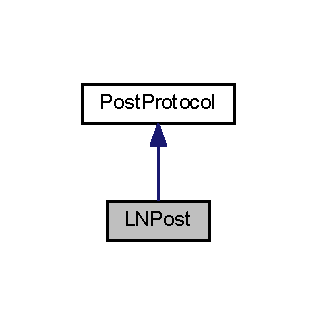
\includegraphics[width=152pt]{class_l_n_post__inherit__graph}
\end{center}
\end{figure}


Collaboration diagram for L\-N\-Post\-:\nopagebreak
\begin{figure}[H]
\begin{center}
\leavevmode
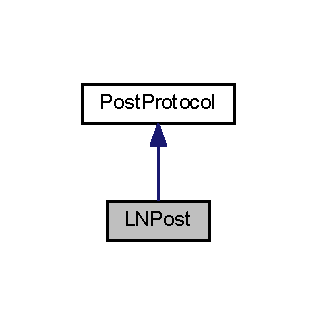
\includegraphics[width=152pt]{class_l_n_post__coll__graph}
\end{center}
\end{figure}
\subsection*{Public Member Functions}
\begin{DoxyCompactItemize}
\item 
void \hyperlink{class_l_n_post_a3ab3b83674e572c7a8c645c8ea6f447d}{novo} (\hyperlink{class_post}{Post})
\begin{DoxyCompactList}\small\item\em Método responsável por criar uma postagem. \end{DoxyCompactList}\item 
void \hyperlink{class_l_n_post_a76e4575cc5e542510c1f135f879e88f5}{update} (\hyperlink{class_post}{Post})
\begin{DoxyCompactList}\small\item\em Método responsável por atualizar uma postagem. \end{DoxyCompactList}\item 
void \hyperlink{class_l_n_post_a24a5694180c400a4f75b05e3cc2b1b49}{deleta} (\hyperlink{class_post}{Post})
\begin{DoxyCompactList}\small\item\em Método responsável por deletar uma postagem. \end{DoxyCompactList}\item 
list$<$ \hyperlink{class_post}{Post} $>$ \hyperlink{class_l_n_post_adb8838a2a49afbc84d17ea8fc4773c7b}{listar} ()
\begin{DoxyCompactList}\small\item\em Método responsável por listar todas as postagens. \end{DoxyCompactList}\item 
list$<$ \hyperlink{class_post}{Post} $>$ \hyperlink{class_l_n_post_ad57f97108f666b1c2cc512e8301bc659}{listar\-Por\-User} (\hyperlink{class_post}{Post})
\begin{DoxyCompactList}\small\item\em Método responsável por listar as postagens por usuário. \end{DoxyCompactList}\item 
\hyperlink{class_post}{Post} \hyperlink{class_l_n_post_acb5f1b004c87e6cc34afa3890ff09682}{pegar} (\hyperlink{class_post}{Post})
\begin{DoxyCompactList}\small\item\em Método responsável por pegar uma postagens. \end{DoxyCompactList}\item 
void \hyperlink{class_l_n_post_a0f45810ec3c120b544810d9408d013e9}{set\-Percistence} (\hyperlink{class_percistence_protocol}{Percistence\-Protocol} $\ast$)
\begin{DoxyCompactList}\small\item\em Método responsável por ativar um protocolo de persitência. \end{DoxyCompactList}\item 
\hypertarget{class_l_n_post_ad3ca792ffe30c002e26008c5d85061eb}{\hyperlink{class_l_n_post_ad3ca792ffe30c002e26008c5d85061eb}{L\-N\-Post} ()}\label{class_l_n_post_ad3ca792ffe30c002e26008c5d85061eb}

\begin{DoxyCompactList}\small\item\em Método responsável por construir a classe. \end{DoxyCompactList}\item 
\hypertarget{class_l_n_post_a227e0227d4ebf74d8a2d55912875fb8d}{\hyperlink{class_l_n_post_a227e0227d4ebf74d8a2d55912875fb8d}{$\sim$\-L\-N\-Post} ()}\label{class_l_n_post_a227e0227d4ebf74d8a2d55912875fb8d}

\begin{DoxyCompactList}\small\item\em Método responsável por construir a classe. \end{DoxyCompactList}\end{DoxyCompactItemize}


\subsection{Member Function Documentation}
\hypertarget{class_l_n_post_a24a5694180c400a4f75b05e3cc2b1b49}{\index{L\-N\-Post@{L\-N\-Post}!deleta@{deleta}}
\index{deleta@{deleta}!LNPost@{L\-N\-Post}}
\subsubsection[{deleta}]{\setlength{\rightskip}{0pt plus 5cm}L\-N\-Post\-::deleta (
\begin{DoxyParamCaption}
\item[{{\bf Post}}]{post}
\end{DoxyParamCaption}
)\hspace{0.3cm}{\ttfamily [virtual]}}}\label{class_l_n_post_a24a5694180c400a4f75b05e3cc2b1b49}


Método responsável por deletar uma postagem. 


\begin{DoxyParams}{Parameters}
{\em \hyperlink{class_post}{Post}} & = objeto de um post \\
\hline
\end{DoxyParams}


Implements \hyperlink{class_post_protocol}{Post\-Protocol}.



Here is the call graph for this function\-:\nopagebreak
\begin{figure}[H]
\begin{center}
\leavevmode
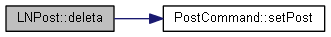
\includegraphics[width=320pt]{class_l_n_post_a24a5694180c400a4f75b05e3cc2b1b49_cgraph}
\end{center}
\end{figure}


\hypertarget{class_l_n_post_adb8838a2a49afbc84d17ea8fc4773c7b}{\index{L\-N\-Post@{L\-N\-Post}!listar@{listar}}
\index{listar@{listar}!LNPost@{L\-N\-Post}}
\subsubsection[{listar}]{\setlength{\rightskip}{0pt plus 5cm}L\-N\-Post\-::listar (
\begin{DoxyParamCaption}
{}
\end{DoxyParamCaption}
)\hspace{0.3cm}{\ttfamily [virtual]}}}\label{class_l_n_post_adb8838a2a49afbc84d17ea8fc4773c7b}


Método responsável por listar todas as postagens. 


\begin{DoxyParams}{Parameters}
{\em \hyperlink{class_post}{Post}} & = objeto de um post \\
\hline
\end{DoxyParams}


Implements \hyperlink{class_post_protocol}{Post\-Protocol}.



Here is the call graph for this function\-:\nopagebreak
\begin{figure}[H]
\begin{center}
\leavevmode
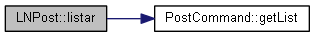
\includegraphics[width=308pt]{class_l_n_post_adb8838a2a49afbc84d17ea8fc4773c7b_cgraph}
\end{center}
\end{figure}


\hypertarget{class_l_n_post_ad57f97108f666b1c2cc512e8301bc659}{\index{L\-N\-Post@{L\-N\-Post}!listar\-Por\-User@{listar\-Por\-User}}
\index{listar\-Por\-User@{listar\-Por\-User}!LNPost@{L\-N\-Post}}
\subsubsection[{listar\-Por\-User}]{\setlength{\rightskip}{0pt plus 5cm}L\-N\-Post\-::listar\-Por\-User (
\begin{DoxyParamCaption}
\item[{{\bf Post}}]{post}
\end{DoxyParamCaption}
)\hspace{0.3cm}{\ttfamily [virtual]}}}\label{class_l_n_post_ad57f97108f666b1c2cc512e8301bc659}


Método responsável por listar as postagens por usuário. 


\begin{DoxyParams}{Parameters}
{\em \hyperlink{class_post}{Post}} & = objeto de um post \\
\hline
\end{DoxyParams}


Implements \hyperlink{class_post_protocol}{Post\-Protocol}.



Here is the call graph for this function\-:\nopagebreak
\begin{figure}[H]
\begin{center}
\leavevmode
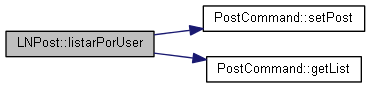
\includegraphics[width=350pt]{class_l_n_post_ad57f97108f666b1c2cc512e8301bc659_cgraph}
\end{center}
\end{figure}


\hypertarget{class_l_n_post_a3ab3b83674e572c7a8c645c8ea6f447d}{\index{L\-N\-Post@{L\-N\-Post}!novo@{novo}}
\index{novo@{novo}!LNPost@{L\-N\-Post}}
\subsubsection[{novo}]{\setlength{\rightskip}{0pt plus 5cm}L\-N\-Post\-::novo (
\begin{DoxyParamCaption}
\item[{{\bf Post}}]{post}
\end{DoxyParamCaption}
)\hspace{0.3cm}{\ttfamily [virtual]}}}\label{class_l_n_post_a3ab3b83674e572c7a8c645c8ea6f447d}


Método responsável por criar uma postagem. 


\begin{DoxyParams}{Parameters}
{\em \hyperlink{class_post}{Post}} & = objeto de um post \\
\hline
\end{DoxyParams}


Implements \hyperlink{class_post_protocol}{Post\-Protocol}.



Here is the call graph for this function\-:\nopagebreak
\begin{figure}[H]
\begin{center}
\leavevmode
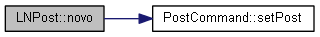
\includegraphics[width=312pt]{class_l_n_post_a3ab3b83674e572c7a8c645c8ea6f447d_cgraph}
\end{center}
\end{figure}


\hypertarget{class_l_n_post_acb5f1b004c87e6cc34afa3890ff09682}{\index{L\-N\-Post@{L\-N\-Post}!pegar@{pegar}}
\index{pegar@{pegar}!LNPost@{L\-N\-Post}}
\subsubsection[{pegar}]{\setlength{\rightskip}{0pt plus 5cm}L\-N\-Post\-::pegar (
\begin{DoxyParamCaption}
\item[{{\bf Post}}]{post}
\end{DoxyParamCaption}
)\hspace{0.3cm}{\ttfamily [virtual]}}}\label{class_l_n_post_acb5f1b004c87e6cc34afa3890ff09682}


Método responsável por pegar uma postagens. 


\begin{DoxyParams}{Parameters}
{\em \hyperlink{class_post}{Post}} & = objeto de um post \\
\hline
\end{DoxyParams}


Implements \hyperlink{class_post_protocol}{Post\-Protocol}.



Here is the call graph for this function\-:\nopagebreak
\begin{figure}[H]
\begin{center}
\leavevmode
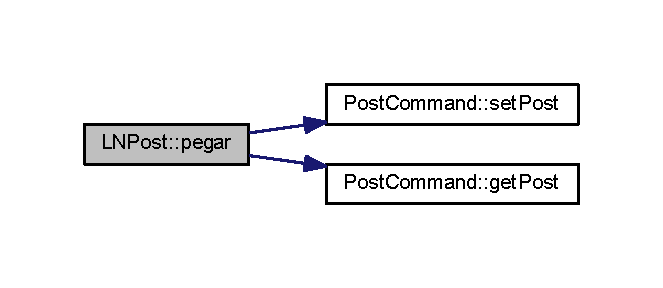
\includegraphics[width=318pt]{class_l_n_post_acb5f1b004c87e6cc34afa3890ff09682_cgraph}
\end{center}
\end{figure}


\hypertarget{class_l_n_post_a0f45810ec3c120b544810d9408d013e9}{\index{L\-N\-Post@{L\-N\-Post}!set\-Percistence@{set\-Percistence}}
\index{set\-Percistence@{set\-Percistence}!LNPost@{L\-N\-Post}}
\subsubsection[{set\-Percistence}]{\setlength{\rightskip}{0pt plus 5cm}L\-N\-Post\-::set\-Percistence (
\begin{DoxyParamCaption}
\item[{{\bf Percistence\-Protocol} $\ast$}]{percistence}
\end{DoxyParamCaption}
)\hspace{0.3cm}{\ttfamily [virtual]}}}\label{class_l_n_post_a0f45810ec3c120b544810d9408d013e9}


Método responsável por ativar um protocolo de persitência. 


\begin{DoxyParams}{Parameters}
{\em \hyperlink{class_percistence_protocol}{Percistence\-Protocol}} & = protocolo de persitência \\
\hline
\end{DoxyParams}


Implements \hyperlink{class_post_protocol}{Post\-Protocol}.

\hypertarget{class_l_n_post_a76e4575cc5e542510c1f135f879e88f5}{\index{L\-N\-Post@{L\-N\-Post}!update@{update}}
\index{update@{update}!LNPost@{L\-N\-Post}}
\subsubsection[{update}]{\setlength{\rightskip}{0pt plus 5cm}L\-N\-Post\-::update (
\begin{DoxyParamCaption}
\item[{{\bf Post}}]{post}
\end{DoxyParamCaption}
)\hspace{0.3cm}{\ttfamily [virtual]}}}\label{class_l_n_post_a76e4575cc5e542510c1f135f879e88f5}


Método responsável por atualizar uma postagem. 


\begin{DoxyParams}{Parameters}
{\em \hyperlink{class_post}{Post}} & = objeto de um post \\
\hline
\end{DoxyParams}


Implements \hyperlink{class_post_protocol}{Post\-Protocol}.



Here is the call graph for this function\-:\nopagebreak
\begin{figure}[H]
\begin{center}
\leavevmode
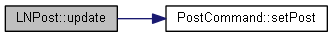
\includegraphics[width=322pt]{class_l_n_post_a76e4575cc5e542510c1f135f879e88f5_cgraph}
\end{center}
\end{figure}




The documentation for this class was generated from the following files\-:\begin{DoxyCompactItemize}
\item 
C\-:/\-Users/\-Vitor/\-Desktop/\-Work\-Space/\-P\-R\-O\-J\-E\-T\-O\-\_\-\-F\-I\-N\-A\-L\-\_\-\-P\-O\-O/\-P\-R\-O\-J\-E\-T\-O\-\_\-\-D\-E\-V/\-P\-R\-O\-J\-E\-T\-O/\-Projeto\-\_\-codeblocks/Log\-Neg.\-h\item 
C\-:/\-Users/\-Vitor/\-Desktop/\-Work\-Space/\-P\-R\-O\-J\-E\-T\-O\-\_\-\-F\-I\-N\-A\-L\-\_\-\-P\-O\-O/\-P\-R\-O\-J\-E\-T\-O\-\_\-\-D\-E\-V/\-P\-R\-O\-J\-E\-T\-O/\-Projeto\-\_\-codeblocks/Log\-Neg.\-cpp\end{DoxyCompactItemize}

\hypertarget{class_l_n_user}{\section{L\-N\-User Class Reference}
\label{class_l_n_user}\index{L\-N\-User@{L\-N\-User}}
}


Essa � a classe respons�vel pela l�gica de neg�cios para uma postagems.  




Inheritance diagram for L\-N\-User\-:
\nopagebreak
\begin{figure}[H]
\begin{center}
\leavevmode
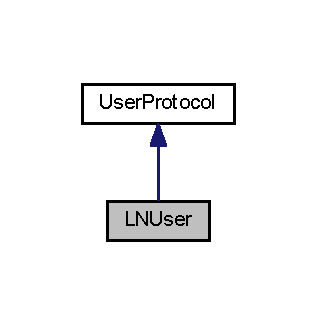
\includegraphics[width=152pt]{class_l_n_user__inherit__graph}
\end{center}
\end{figure}


Collaboration diagram for L\-N\-User\-:
\nopagebreak
\begin{figure}[H]
\begin{center}
\leavevmode
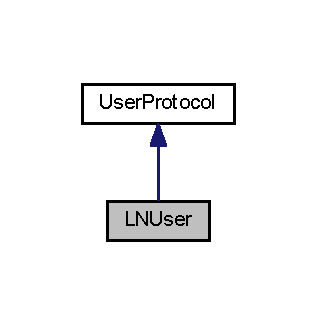
\includegraphics[width=152pt]{class_l_n_user__coll__graph}
\end{center}
\end{figure}
\subsection*{Public Member Functions}
\begin{DoxyCompactItemize}
\item 
void \hyperlink{class_l_n_user_a74c91c7a9e6d8ceaf8ebfed027178221}{autenticar} (User)
\begin{DoxyCompactList}\small\item\em M�todo respons�vel por autenticar um usu�rio. \end{DoxyCompactList}\item 
void \hyperlink{class_l_n_user_a4702a50096c617aa7a9ea9b25fda3063}{cadastrar} (User)
\begin{DoxyCompactList}\small\item\em M�todo respons�vel por cadastar um usu�rio. \end{DoxyCompactList}\item 
void \hyperlink{class_l_n_user_a4093083f84eec431151c7315b5064b88}{update} (User)
\begin{DoxyCompactList}\small\item\em M�todo respons�vel por atualizar um usu�rio. \end{DoxyCompactList}\item 
void \hyperlink{class_l_n_user_ac2058724d8d0b2ab8da440b9acc2b80a}{deletar} (User)
\begin{DoxyCompactList}\small\item\em M�todo respons�vel por deletar um usu�rio. \end{DoxyCompactList}\item 
\hypertarget{class_l_n_user_a49a8cb98850d1812aa504fd7ec1c64f0}{list$<$ User $>$ \hyperlink{class_l_n_user_a49a8cb98850d1812aa504fd7ec1c64f0}{Listar} ()}\label{class_l_n_user_a49a8cb98850d1812aa504fd7ec1c64f0}

\begin{DoxyCompactList}\small\item\em M�todo respons�vel por listar os usu�rios. \end{DoxyCompactList}\item 
void \hyperlink{class_l_n_user_aadeddd422a7e5b1b7059b472dcee1631}{set\-Percistence} (Percistence\-Protocol $\ast$)
\begin{DoxyCompactList}\small\item\em M�todo respons�vel por ativar um protocolo de persit�ncia. \end{DoxyCompactList}\item 
\hypertarget{class_l_n_user_aacf199ac94fc28825e3692aa097fe842}{\hyperlink{class_l_n_user_aacf199ac94fc28825e3692aa097fe842}{L\-N\-User} ()}\label{class_l_n_user_aacf199ac94fc28825e3692aa097fe842}

\begin{DoxyCompactList}\small\item\em M�todo respons�vel por construir a classe. \end{DoxyCompactList}\item 
\hypertarget{class_l_n_user_a980d1a92278869298b21acd8871854bd}{\hyperlink{class_l_n_user_a980d1a92278869298b21acd8871854bd}{$\sim$\-L\-N\-User} ()}\label{class_l_n_user_a980d1a92278869298b21acd8871854bd}

\begin{DoxyCompactList}\small\item\em M�todo respons�vel por descontruir a classe. \end{DoxyCompactList}\end{DoxyCompactItemize}


\subsection{Detailed Description}
Essa � a classe respons�vel pela l�gica de neg�cios para uma postagems. 

\subsection{Member Function Documentation}
\hypertarget{class_l_n_user_a74c91c7a9e6d8ceaf8ebfed027178221}{\index{L\-N\-User@{L\-N\-User}!autenticar@{autenticar}}
\index{autenticar@{autenticar}!LNUser@{L\-N\-User}}
\subsubsection[{autenticar}]{\setlength{\rightskip}{0pt plus 5cm}L\-N\-User\-::autenticar (
\begin{DoxyParamCaption}
\item[{User}]{}
\end{DoxyParamCaption}
)}}\label{class_l_n_user_a74c91c7a9e6d8ceaf8ebfed027178221}


M�todo respons�vel por autenticar um usu�rio. 


\begin{DoxyParams}{Parameters}
{\em User} & = objeto de um usu�rio \\
\hline
\end{DoxyParams}
\hypertarget{class_l_n_user_a4702a50096c617aa7a9ea9b25fda3063}{\index{L\-N\-User@{L\-N\-User}!cadastrar@{cadastrar}}
\index{cadastrar@{cadastrar}!LNUser@{L\-N\-User}}
\subsubsection[{cadastrar}]{\setlength{\rightskip}{0pt plus 5cm}L\-N\-User\-::cadastrar (
\begin{DoxyParamCaption}
\item[{User}]{}
\end{DoxyParamCaption}
)}}\label{class_l_n_user_a4702a50096c617aa7a9ea9b25fda3063}


M�todo respons�vel por cadastar um usu�rio. 


\begin{DoxyParams}{Parameters}
{\em User} & = objeto de um usu�rio \\
\hline
\end{DoxyParams}
\hypertarget{class_l_n_user_ac2058724d8d0b2ab8da440b9acc2b80a}{\index{L\-N\-User@{L\-N\-User}!deletar@{deletar}}
\index{deletar@{deletar}!LNUser@{L\-N\-User}}
\subsubsection[{deletar}]{\setlength{\rightskip}{0pt plus 5cm}L\-N\-User\-::deletar (
\begin{DoxyParamCaption}
\item[{User}]{}
\end{DoxyParamCaption}
)}}\label{class_l_n_user_ac2058724d8d0b2ab8da440b9acc2b80a}


M�todo respons�vel por deletar um usu�rio. 


\begin{DoxyParams}{Parameters}
{\em User} & = objeto de um usu�rio \\
\hline
\end{DoxyParams}
\hypertarget{class_l_n_user_aadeddd422a7e5b1b7059b472dcee1631}{\index{L\-N\-User@{L\-N\-User}!set\-Percistence@{set\-Percistence}}
\index{set\-Percistence@{set\-Percistence}!LNUser@{L\-N\-User}}
\subsubsection[{set\-Percistence}]{\setlength{\rightskip}{0pt plus 5cm}L\-N\-User\-::set\-Percistence (
\begin{DoxyParamCaption}
\item[{Percistence\-Protocol $\ast$}]{}
\end{DoxyParamCaption}
)\hspace{0.3cm}{\ttfamily [inline]}}}\label{class_l_n_user_aadeddd422a7e5b1b7059b472dcee1631}


M�todo respons�vel por ativar um protocolo de persit�ncia. 


\begin{DoxyParams}{Parameters}
{\em Percistence\-Protocol} & = protocolo de persit�ncia \\
\hline
\end{DoxyParams}
\hypertarget{class_l_n_user_a4093083f84eec431151c7315b5064b88}{\index{L\-N\-User@{L\-N\-User}!update@{update}}
\index{update@{update}!LNUser@{L\-N\-User}}
\subsubsection[{update}]{\setlength{\rightskip}{0pt plus 5cm}L\-N\-User\-::update (
\begin{DoxyParamCaption}
\item[{User}]{}
\end{DoxyParamCaption}
)}}\label{class_l_n_user_a4093083f84eec431151c7315b5064b88}


M�todo respons�vel por atualizar um usu�rio. 


\begin{DoxyParams}{Parameters}
{\em User} & = objeto de um usu�rio \\
\hline
\end{DoxyParams}


The documentation for this class was generated from the following file\-:\begin{DoxyCompactItemize}
\item 
Stub\-L\-N.\-cpp\end{DoxyCompactItemize}

\hypertarget{class_logic_error}{\section{Logic\-Error Class Reference}
\label{class_logic_error}\index{Logic\-Error@{Logic\-Error}}
}


Essa é a classe responsável por gerir os erros que podem aparecer na camada de persitência.  




{\ttfamily \#include $<$Errors.\-h$>$}

\subsection*{Public Member Functions}
\begin{DoxyCompactItemize}
\item 
\hypertarget{class_logic_error_adb9f58f48bbfaf0e33f04a2fe4a579b3}{string \hyperlink{class_logic_error_adb9f58f48bbfaf0e33f04a2fe4a579b3}{what} ()}\label{class_logic_error_adb9f58f48bbfaf0e33f04a2fe4a579b3}

\begin{DoxyCompactList}\small\item\em Funcao que recebe o erro da camada lógica de negócio. \end{DoxyCompactList}\item 
\hyperlink{class_logic_error_afd70216c2cb88abd86db74d419a8b62e}{Logic\-Error} (string)
\begin{DoxyCompactList}\small\item\em Funcao que descobre o que o erro enviado pela lógica de negócio significa. \end{DoxyCompactList}\end{DoxyCompactItemize}


\subsection{Detailed Description}
Essa é a classe responsável por gerir os erros que podem aparecer na camada de persitência. 

\subsection{Constructor \& Destructor Documentation}
\hypertarget{class_logic_error_afd70216c2cb88abd86db74d419a8b62e}{\index{Logic\-Error@{Logic\-Error}!Logic\-Error@{Logic\-Error}}
\index{Logic\-Error@{Logic\-Error}!LogicError@{Logic\-Error}}
\subsubsection[{Logic\-Error}]{\setlength{\rightskip}{0pt plus 5cm}Logic\-Error\-::\-Logic\-Error (
\begin{DoxyParamCaption}
\item[{string}]{erro}
\end{DoxyParamCaption}
)\hspace{0.3cm}{\ttfamily [inline]}}}\label{class_logic_error_afd70216c2cb88abd86db74d419a8b62e}


Funcao que descobre o que o erro enviado pela lógica de negócio significa. 


\begin{DoxyParams}{Parameters}
{\em string} & \-: erro da lógica de negócio. \\
\hline
\end{DoxyParams}


The documentation for this class was generated from the following file\-:\begin{DoxyCompactItemize}
\item 
\hyperlink{_errors_8h}{Errors.\-h}\end{DoxyCompactItemize}

\hypertarget{class_percistence_error}{\section{Percistence\-Error Class Reference}
\label{class_percistence_error}\index{Percistence\-Error@{Percistence\-Error}}
}


Essa é a classe responsável por gerir os erros que podem aparecer na camada de persitência.  




{\ttfamily \#include $<$Errors.\-h$>$}

\subsection*{Public Member Functions}
\begin{DoxyCompactItemize}
\item 
\hypertarget{class_percistence_error_ab6696d7321429f1c4cce537e93937a90}{string \hyperlink{class_percistence_error_ab6696d7321429f1c4cce537e93937a90}{what} ()}\label{class_percistence_error_ab6696d7321429f1c4cce537e93937a90}

\begin{DoxyCompactList}\small\item\em Funcao que recebe o erro da camada de persistência. \end{DoxyCompactList}\item 
\hyperlink{class_percistence_error_ac94a0128b5061037192e4ad9f7892c7b}{Percistence\-Error} (string)
\begin{DoxyCompactList}\small\item\em Funcao que descobre o que o erro enviado pela persitência significa. \end{DoxyCompactList}\end{DoxyCompactItemize}


\subsection{Detailed Description}
Essa é a classe responsável por gerir os erros que podem aparecer na camada de persitência. 

\subsection{Constructor \& Destructor Documentation}
\hypertarget{class_percistence_error_ac94a0128b5061037192e4ad9f7892c7b}{\index{Percistence\-Error@{Percistence\-Error}!Percistence\-Error@{Percistence\-Error}}
\index{Percistence\-Error@{Percistence\-Error}!PercistenceError@{Percistence\-Error}}
\subsubsection[{Percistence\-Error}]{\setlength{\rightskip}{0pt plus 5cm}Percistence\-Error\-::\-Percistence\-Error (
\begin{DoxyParamCaption}
\item[{string}]{erro}
\end{DoxyParamCaption}
)\hspace{0.3cm}{\ttfamily [inline]}}}\label{class_percistence_error_ac94a0128b5061037192e4ad9f7892c7b}


Funcao que descobre o que o erro enviado pela persitência significa. 


\begin{DoxyParams}{Parameters}
{\em string} & \-: erro da lógica da persistência. \\
\hline
\end{DoxyParams}


The documentation for this class was generated from the following file\-:\begin{DoxyCompactItemize}
\item 
\hyperlink{_errors_8h}{Errors.\-h}\end{DoxyCompactItemize}

\hypertarget{class_percistence_protocol}{\section{Percistence\-Protocol Class Reference}
\label{class_percistence_protocol}\index{Percistence\-Protocol@{Percistence\-Protocol}}
}
\subsection*{Public Member Functions}
\begin{DoxyCompactItemize}
\item 
\hypertarget{class_percistence_protocol_aabb1342054dba836dfd026254dbffafb}{virtual void \hyperlink{class_percistence_protocol_aabb1342054dba836dfd026254dbffafb}{exec} (A\-Command $\ast$)=0  throw (\-Percistence\-Error)}\label{class_percistence_protocol_aabb1342054dba836dfd026254dbffafb}

\begin{DoxyCompactList}\small\item\em executar um comando abstrato implementando design pattern command \end{DoxyCompactList}\item 
\hypertarget{class_percistence_protocol_ad68bcb2a3e256694b59cafa2fcf43606}{virtual \hyperlink{class_percistence_protocol_ad68bcb2a3e256694b59cafa2fcf43606}{$\sim$\-Percistence\-Protocol} ()}\label{class_percistence_protocol_ad68bcb2a3e256694b59cafa2fcf43606}

\begin{DoxyCompactList}\small\item\em Destruidora do protocolo. \end{DoxyCompactList}\end{DoxyCompactItemize}


The documentation for this class was generated from the following file\-:\begin{DoxyCompactItemize}
\item 
\hyperlink{_percistence_protocol_8h}{Percistence\-Protocol.\-h}\end{DoxyCompactItemize}

\hypertarget{class_persistence_protocol}{\section{Persistence\-Protocol Class Reference}
\label{class_persistence_protocol}\index{Persistence\-Protocol@{Persistence\-Protocol}}
}


Essa e a classe responsavel por criar um protocolo de persitência.  




{\ttfamily \#include $<$Percistence\-Protocol.\-h$>$}



\subsection{Detailed Description}
Essa e a classe responsavel por criar um protocolo de persitência. 

The documentation for this class was generated from the following file\-:\begin{DoxyCompactItemize}
\item 
\hyperlink{_percistence_protocol_8h}{Percistence\-Protocol.\-h}\end{DoxyCompactItemize}

\hypertarget{class_post_protocol}{\section{Post\-Protocol Class Reference}
\label{class_post_protocol}\index{Post\-Protocol@{Post\-Protocol}}
}


Inheritance diagram for Post\-Protocol\-:\nopagebreak
\begin{figure}[H]
\begin{center}
\leavevmode
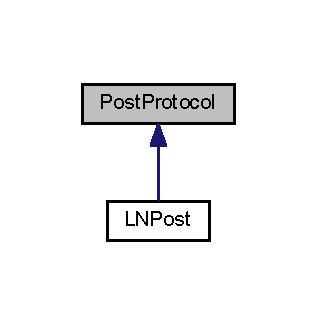
\includegraphics[width=152pt]{class_post_protocol__inherit__graph}
\end{center}
\end{figure}
\subsection*{Public Member Functions}
\begin{DoxyCompactItemize}
\item 
\hypertarget{class_post_protocol_a29c8f475d6c5f284ad94d51aeaf0428a}{virtual void {\bfseries novo} (Post)=0}\label{class_post_protocol_a29c8f475d6c5f284ad94d51aeaf0428a}

\item 
\hypertarget{class_post_protocol_a7cac627996f60cc8d3a3ac79541906da}{virtual void {\bfseries update} (Post)=0}\label{class_post_protocol_a7cac627996f60cc8d3a3ac79541906da}

\item 
\hypertarget{class_post_protocol_ada9f6161a46b9adf85b404785e18becd}{virtual void {\bfseries deleta} (Post)=0}\label{class_post_protocol_ada9f6161a46b9adf85b404785e18becd}

\item 
\hypertarget{class_post_protocol_a590d2c0f349b99a33e69661fffdc078e}{virtual list$<$ Post $>$ {\bfseries listar} ()=0}\label{class_post_protocol_a590d2c0f349b99a33e69661fffdc078e}

\item 
\hypertarget{class_post_protocol_addfc8f6b5ffd5af04f0ef6a1a3b7d8f1}{virtual list$<$ Post $>$ {\bfseries listar\-Por\-User} (Post)=0}\label{class_post_protocol_addfc8f6b5ffd5af04f0ef6a1a3b7d8f1}

\item 
\hypertarget{class_post_protocol_a6455f6e36f21ba008e3529e77185d884}{virtual Post {\bfseries pegar} (Post)=0}\label{class_post_protocol_a6455f6e36f21ba008e3529e77185d884}

\item 
\hypertarget{class_post_protocol_a9ed7d312b4726aba6bc880d90ec844a7}{virtual void {\bfseries set\-Percistence} (\hyperlink{class_percistence_protocol}{Percistence\-Protocol} $\ast$)=0}\label{class_post_protocol_a9ed7d312b4726aba6bc880d90ec844a7}

\end{DoxyCompactItemize}


The documentation for this class was generated from the following file\-:\begin{DoxyCompactItemize}
\item 
\hyperlink{_protocolo_l_n_8h}{Protocolo\-L\-N.\-h}\end{DoxyCompactItemize}

\hypertarget{class_user_protocol}{\section{User\-Protocol Class Reference}
\label{class_user_protocol}\index{User\-Protocol@{User\-Protocol}}
}


Protocolo de controle da controladora de usuario.  




{\ttfamily \#include $<$Protocolo\-L\-N.\-h$>$}



Inheritance diagram for User\-Protocol\-:\nopagebreak
\begin{figure}[H]
\begin{center}
\leavevmode
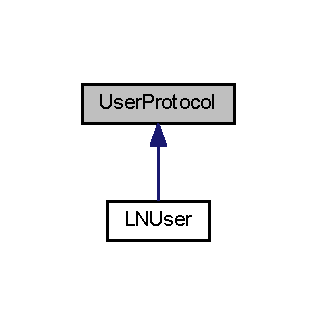
\includegraphics[width=152pt]{class_user_protocol__inherit__graph}
\end{center}
\end{figure}
\subsection*{Public Member Functions}
\begin{DoxyCompactItemize}
\item 
\hypertarget{class_user_protocol_a848b4c9ad3b03384da94606c8f3f39f4}{virtual void {\bfseries autenticar} (\hyperlink{class_user}{User})=0}\label{class_user_protocol_a848b4c9ad3b03384da94606c8f3f39f4}

\item 
\hypertarget{class_user_protocol_a82ef4359d21dea2516370077eebc191f}{virtual void {\bfseries cadastrar} (\hyperlink{class_user}{User})=0}\label{class_user_protocol_a82ef4359d21dea2516370077eebc191f}

\item 
\hypertarget{class_user_protocol_a763b2abc464281839f982e6a33a19ebf}{virtual void {\bfseries update} (\hyperlink{class_user}{User})=0}\label{class_user_protocol_a763b2abc464281839f982e6a33a19ebf}

\item 
\hypertarget{class_user_protocol_a60d2fcc3efc076fadd2463980439652e}{virtual void {\bfseries deletar} (\hyperlink{class_user}{User})=0}\label{class_user_protocol_a60d2fcc3efc076fadd2463980439652e}

\item 
\hypertarget{class_user_protocol_a4da9152e6f9f128fb37467c8ee3cdca9}{virtual list$<$ \hyperlink{class_user}{User} $>$ {\bfseries Listar} ()=0}\label{class_user_protocol_a4da9152e6f9f128fb37467c8ee3cdca9}

\item 
\hypertarget{class_user_protocol_acf8d6fb7d463085084cb428ec316d23a}{virtual void {\bfseries set\-Percistence} (\hyperlink{class_percistence_protocol}{Percistence\-Protocol} $\ast$)=0}\label{class_user_protocol_acf8d6fb7d463085084cb428ec316d23a}

\end{DoxyCompactItemize}


\subsection{Detailed Description}
Protocolo de controle da controladora de usuario. 

The documentation for this class was generated from the following file\-:\begin{DoxyCompactItemize}
\item 
C\-:/\-Users/\-Vitor/\-Desktop/\-Work\-Space/\-P\-R\-O\-J\-E\-T\-O\-\_\-\-F\-I\-N\-A\-L\-\_\-\-P\-O\-O/\-P\-R\-O\-J\-E\-T\-O\-\_\-\-D\-E\-V/\-P\-R\-O\-J\-E\-T\-O/\-Projeto\-\_\-codeblocks/\hyperlink{_protocolo_l_n_8h}{Protocolo\-L\-N.\-h}\end{DoxyCompactItemize}

\chapter{File Documentation}
\hypertarget{_errors_8h}{\section{C\-:/\-Users/\-Vitor/\-Desktop/\-Work\-Space/\-P\-R\-O\-J\-E\-T\-O\-\_\-\-F\-I\-N\-A\-L\-\_\-\-P\-O\-O/\-P\-R\-O\-J\-E\-T\-O\-\_\-\-D\-E\-V/\-P\-R\-O\-J\-E\-T\-O/\-Projeto\-\_\-codeblocks/\-Errors.h File Reference}
\label{_errors_8h}\index{C\-:/\-Users/\-Vitor/\-Desktop/\-Work\-Space/\-P\-R\-O\-J\-E\-T\-O\-\_\-\-F\-I\-N\-A\-L\-\_\-\-P\-O\-O/\-P\-R\-O\-J\-E\-T\-O\-\_\-\-D\-E\-V/\-P\-R\-O\-J\-E\-T\-O/\-Projeto\-\_\-codeblocks/\-Errors.\-h@{C\-:/\-Users/\-Vitor/\-Desktop/\-Work\-Space/\-P\-R\-O\-J\-E\-T\-O\-\_\-\-F\-I\-N\-A\-L\-\_\-\-P\-O\-O/\-P\-R\-O\-J\-E\-T\-O\-\_\-\-D\-E\-V/\-P\-R\-O\-J\-E\-T\-O/\-Projeto\-\_\-codeblocks/\-Errors.\-h}}
}


Este e o cabecalho do modulo das classes entidades que definem as \par
 entidades do sistema neste caso estes sao\-:\par
.  


{\ttfamily \#include $<$string$>$}\\*
Include dependency graph for Errors.\-h\-:
\nopagebreak
\begin{figure}[H]
\begin{center}
\leavevmode
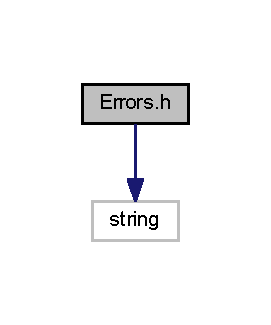
\includegraphics[width=244pt]{_errors_8h__incl}
\end{center}
\end{figure}
This graph shows which files directly or indirectly include this file\-:
\nopagebreak
\begin{figure}[H]
\begin{center}
\leavevmode
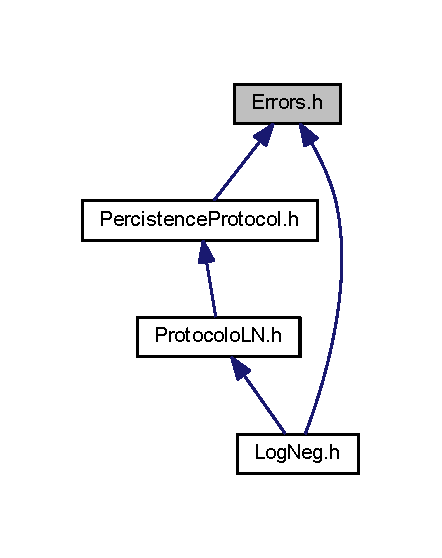
\includegraphics[width=350pt]{_errors_8h__dep__incl}
\end{center}
\end{figure}
\subsection*{Classes}
\begin{DoxyCompactItemize}
\item 
class \hyperlink{class_percistence_error}{Percistence\-Error}
\begin{DoxyCompactList}\small\item\em Essa é a classe responsável por gerir os erros que podem aparecer na camada de persitência. \end{DoxyCompactList}\item 
class \hyperlink{class_logic_error}{Logic\-Error}
\begin{DoxyCompactList}\small\item\em Essa é a classe responsável por gerir os erros que podem aparecer na camada de persitência. \end{DoxyCompactList}\end{DoxyCompactItemize}


\subsection{Detailed Description}
Este e o cabecalho do modulo das classes entidades que definem as \par
 entidades do sistema neste caso estes sao\-:\par
. 
\hypertarget{_percistence_protocol_8h}{\section{Percistence\-Protocol.\-h File Reference}
\label{_percistence_protocol_8h}\index{Percistence\-Protocol.\-h@{Percistence\-Protocol.\-h}}
}


Este e o cabecalho do \par
 protocolo de persistencia.\par
.  


{\ttfamily \#include \char`\"{}Comand.\-h\char`\"{}}\\*
{\ttfamily \#include \char`\"{}Errors.\-h\char`\"{}}\\*
Include dependency graph for Percistence\-Protocol.\-h\-:
\nopagebreak
\begin{figure}[H]
\begin{center}
\leavevmode
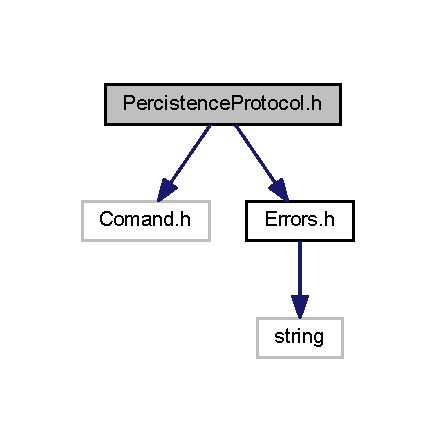
\includegraphics[width=333pt]{_percistence_protocol_8h__incl}
\end{center}
\end{figure}
This graph shows which files directly or indirectly include this file\-:
\nopagebreak
\begin{figure}[H]
\begin{center}
\leavevmode
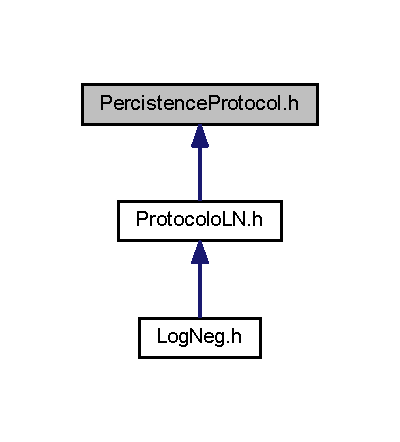
\includegraphics[width=192pt]{_percistence_protocol_8h__dep__incl}
\end{center}
\end{figure}
\subsection*{Classes}
\begin{DoxyCompactItemize}
\item 
class \hyperlink{class_percistence_protocol}{Percistence\-Protocol}
\end{DoxyCompactItemize}


\subsection{Detailed Description}
Este e o cabecalho do \par
 protocolo de persistencia.\par
. 
\hypertarget{_protocolo_l_n_8h}{\section{C\-:/\-Users/\-Vitor/\-Desktop/\-Work\-Space/\-P\-R\-O\-J\-E\-T\-O\-\_\-\-F\-I\-N\-A\-L\-\_\-\-P\-O\-O/\-P\-R\-O\-J\-E\-T\-O\-\_\-\-D\-E\-V/\-P\-R\-O\-J\-E\-T\-O/\-Projeto\-\_\-codeblocks/\-Protocolo\-L\-N.h File Reference}
\label{_protocolo_l_n_8h}\index{C\-:/\-Users/\-Vitor/\-Desktop/\-Work\-Space/\-P\-R\-O\-J\-E\-T\-O\-\_\-\-F\-I\-N\-A\-L\-\_\-\-P\-O\-O/\-P\-R\-O\-J\-E\-T\-O\-\_\-\-D\-E\-V/\-P\-R\-O\-J\-E\-T\-O/\-Projeto\-\_\-codeblocks/\-Protocolo\-L\-N.\-h@{C\-:/\-Users/\-Vitor/\-Desktop/\-Work\-Space/\-P\-R\-O\-J\-E\-T\-O\-\_\-\-F\-I\-N\-A\-L\-\_\-\-P\-O\-O/\-P\-R\-O\-J\-E\-T\-O\-\_\-\-D\-E\-V/\-P\-R\-O\-J\-E\-T\-O/\-Projeto\-\_\-codeblocks/\-Protocolo\-L\-N.\-h}}
}


Este e o cabecalho do modulo da classe Protocolo\-L\-N \par
 respons�vel por implementar os protocolos das controladoras \par
.  


{\ttfamily \#include \char`\"{}Entidades.\-h\char`\"{}}\\*
{\ttfamily \#include \char`\"{}Percistence\-Protocol.\-h\char`\"{}}\\*
{\ttfamily \#include $<$list$>$}\\*
Include dependency graph for Protocolo\-L\-N.\-h\-:
\nopagebreak
\begin{figure}[H]
\begin{center}
\leavevmode
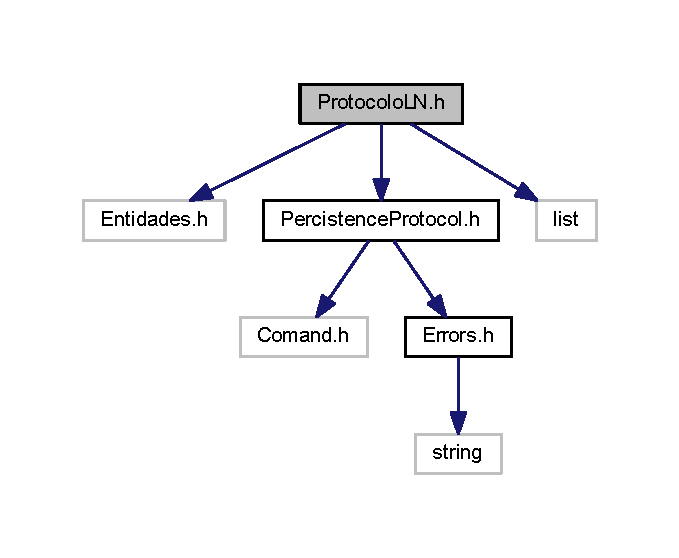
\includegraphics[width=350pt]{_protocolo_l_n_8h__incl}
\end{center}
\end{figure}
This graph shows which files directly or indirectly include this file\-:
\nopagebreak
\begin{figure}[H]
\begin{center}
\leavevmode
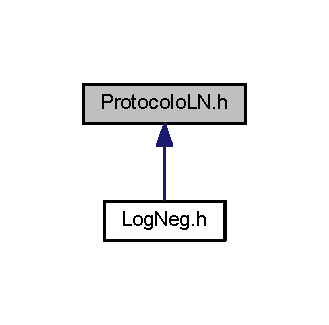
\includegraphics[width=350pt]{_protocolo_l_n_8h__dep__incl}
\end{center}
\end{figure}
\subsection*{Classes}
\begin{DoxyCompactItemize}
\item 
class \hyperlink{class_user_protocol}{User\-Protocol}
\begin{DoxyCompactList}\small\item\em Protocolo de controle da controladora de usuario. \end{DoxyCompactList}\item 
class \hyperlink{class_post_protocol}{Post\-Protocol}
\item 
class \hyperlink{class_coment_protocol}{Coment\-Protocol}
\end{DoxyCompactItemize}


\subsection{Detailed Description}
Este e o cabecalho do modulo da classe Protocolo\-L\-N \par
 respons�vel por implementar os protocolos das controladoras \par
. 
\addcontentsline{toc}{part}{Index}
\printindex
\end{document}
